\section{Introducci'on}
\label{sec:introduccion}


Con la reciente globalizaci'on y auge de internet, idiomas poco representados
en la poblaci'on mundial como es el caso del japon'es han ido ganando seguidores entre
los m'as j'ovenes. El inter'es en pa'ises como Jap'on, Corea o Taiw'an
ha llegado a todo el mundo gracias a series de televisi'on, m'usica, c'omics, videojuegos
y otras muchas formas de ocio.

Sin embargo, la gran diferencia entre estos idiomas y los m'as familiares como el espa'nol,
ingl'es o franc'es hace que su aprendizaje sea especialmente complicado para alguien
que no se dedique exclusivamente al estudio de dichos lenguajes. Adem'as, el hecho de que
el inter'es en estos idiomas es relativamente reciente implica que su estudio no est'e contemplado, en general, 
por academias y universidades, de forma que aquellas personas que deseen comenzar a estudiarlos
deben ser obligatoriamente autodidactas.

Si bien existen ya distintas alternativas en la red para aprender idiomas en general, incluyendo,
por ejemplo, el japon'es, todas siguen el mismo patr'on de ense'nanza para todos los idiomas
por igual, lo cual creemos que no es una soluci'on pr'actica a la hora de ense'nar lenguajes
tan distintos entre s'i.

Este proyecto propone crear un curso espec'ifico de japon'es de forma interactiva, donde
los usuarios puedan aprender el idioma desde las lecciones m'as b'asicas, como pueden ser la
escritura y la pronunciaci'on, hasta conceptos m'as complejos como la propia cultura del pa'is.


\subsection{Justificaci'on y descripci'on del proyecto}
\label{sub:justificacion_y_descripcion_del_proyecto}

Aunque hoy en d'ia ya existen cursos de japon'es online, la mayor'ia de 'estos se basan en lecciones
te'oricas donde el usuario se limita a leer y memorizar. Adem'as, muchos de estos cursos suponen
que los estudiantes ya conocen la escritura y la pronunciaci'on del idioma de antemano, centr'andose
as'i en aspectos m'as avanzados.

En este proyecto se pretende realizar un curso de idioma japon'es compuesto por un conjunto de aplicaciones
web para que los usuarios puedan aprender interactivamente en lugar de 'unicamente
leyendo teor'ia, a la vez que se entretienen. Dichas aplicaciones estar'an
agrupadas en una comunidad online donde todos los usuarios podr'an entablar relaci'on y
comparar las puntuaciones obtenidas en las aplicaciones del curso. El dise'no se har'a de tal
forma que en un futuro las aplicaciones desarrolladas puedan ser adaptadas para aprender
otros idiomas.

Hemos estado interesados en aprender este idioma desde hace varios a'nos y,
aunque hemos encontrado recursos online para aprenderlo, dichos recursos se encontraban
muy dispersos por la red: distintos sitios, distintos formatos y distintos fines. Nuestra
motivaci'on es 'esta, agrupar todo el contenido necesario para aprender el idioma en un solo
lugar y adem'as hacerlo de una forma con la que el usuario pueda aprender divirti'endose, puesto que
'esta es la mejor manera de aprender.

Pretendemos incluir elementos para dar un aire de competitividad a las aplicaciones, ya sea
mediante logros, puntuaciones, rankings u otros m'etodos para hacer que el aprendizaje del
usuario no sea totalmente en solitario, si no que pueda intercambiar experiencias con otros
usuarios. Se registrar'an datos del uso de las aplicaciones para
cada usuario por separado de forma que se pueda guiar u ofrecer consejos personalizados.

\subsection{Motivaci'on}
\label{sub:motivacion}

Este proyecto cubre los tres objetivos principales que ambos autores compart'iamos:
\begin{itemize}
 \item Aprender tecnolog'ias nuevas. Este proyecto se est'a desarrollando utilizando
 herramientas y tecnolog'ias con las que no tenemos ninguna experiencia, por el simple
 hecho de aprender cosas nuevas que puedan resultarnos 'utiles en el futuro. Por esto mismo,
 en muchas ocasiones no escogeremos el camino sencillo y directo para realizar una tarea concreta,
 si no que buscaremos una forma de hacerla que nos aporte nuevos conocimientos.
 \item Aprender nuevos idiomas. Se comenz'o este proyecto con conocimientos muy limitados del
 idioma japon'es, y poco a poco vamos aprendiendo este idioma conforme avanza el desarrollo.
 \item Crear una plataforma que resulte 'util a un n'umero elevado de personas. Como ya se ha explicado,
 en a'nos recientes los idiomas asi'aticos han ganado muchos adeptos, por lo que el p'ublico potencial
 de este proyecto es muy elevado.
\end{itemize}


\subsection{Alternativas}
\label{sub:alternativas}
Algunas de las herramientas m'as famosas que podemos encontrar por internet para aprender idiomas son las siguientes:
\begin{itemize}
 \item Busuu\footnote{\url{http://www.busuu.com/}}

 \begin{center}
 
\includegraphics[width=0.3\textwidth]{busuu}
 \end{center}

 Permite aprender muchos idiomas, incluyendo japon'es, de forma gen'erica ( no espec'ifica para cada idioma). Es un servicio de pago.
 \item Livemocha\footnote{\url{http://livemocha.com/}}

 \begin{center}
 
\includegraphics[width=0.3\textwidth]{livemocha}
 \end{center}

 Como la anterior, tambi'en incluye herramientas 'utiles para aprender japon'es, pero vuelve a ser un servicio de pago.
 \item Duolingo\footnote{\url{https://www.duolingo.com/}}
 
 \begin{center}
 
\includegraphics[width=0.3\textwidth]{duolingo}
 \end{center}
 
 Presenta una forma de aprendizaje por repetici'on muy interesante, pero de momento no incluye el idioma japon'es.
 \item Kanjidamage\footnote{\url{http://kanjidamage.com/}}
 
 \begin{center}
 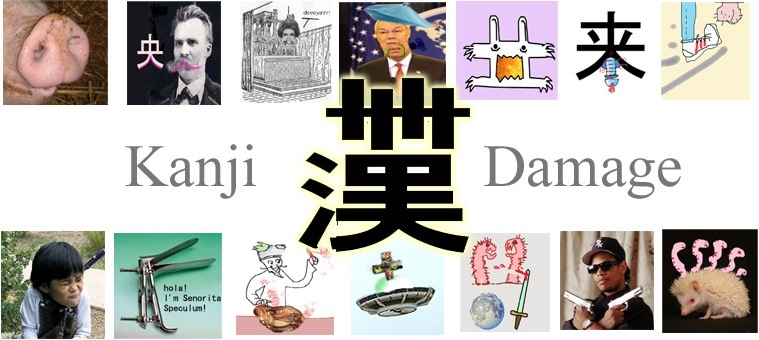
\includegraphics[width=0.3\textwidth]{kanjidamage}
 \end{center}
 
 Aunque muy 'util, se centra exclusivamente en ense'nar una sola parte del idioma japon'es, los kanjis.
\end{itemize}


\subsection{Alcance del proyecto}
\label{sub:alcance_del_proyecto}
Como puede suponerse, la ense'nanza de un idioma al completo mediante aplicaciones interactivas no es
una tarea trivial, sobretodo teniendo en cuenta la poca experiencia de los autores tanto con el idioma
como con las tecnolog'ias utilizadas. Por lo tanto, este Proyecto de Fin de Carrera no pretende abarcar todo el
curso del idioma japon'es ni todas las caracter'isticas que deber'ia tener un curso profesional.
Este PFC se enfoca en la iniciaci'on a este idioma con aplicaciones pensadas para poder familiarizarse
con su escritura y pronunciaci'on. No obstante, este PFC es solamente el inicio de un proyecto en el que
esperamos seguir trabajando durante los pr'oximos a'nos.

